\section{Introduction}
\label{sec:intro}

%!TEX root = ../../main.tex
\begin{figure*}[!t]
    \centering 
    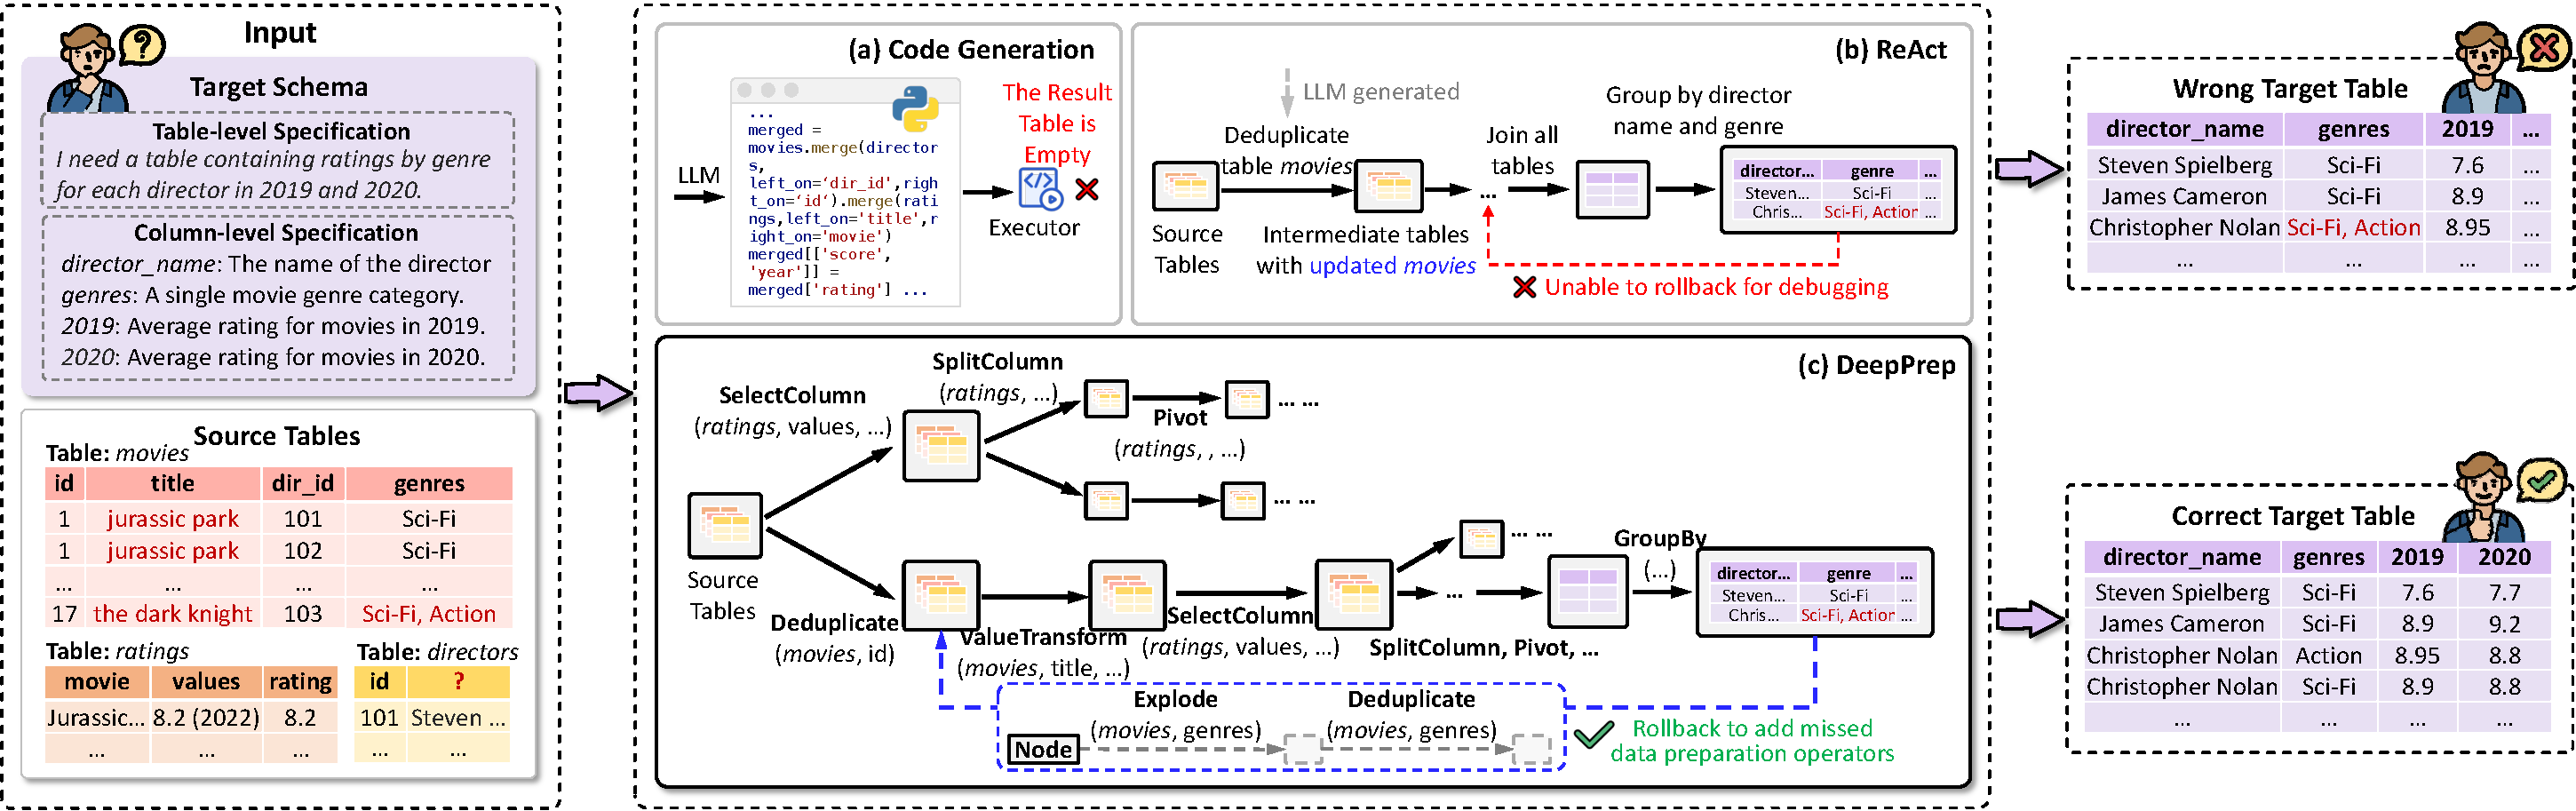
\includegraphics[width=0.95\textwidth]{figures/fig/introduction_example.pdf}
    \vspace{-1em}
    \caption{An illustrative example highlighting the core idea of \sys.
(a) Code generation makes decisions without grounding in intermediate execution results.
(b) ReAct-style approaches follow linear reasoning with limited ability to revise earlier decisions.
(c) \sys applies a tree-based structured exploration, which enables backtracking to resolve non-local errors.
    }
    \label{fig:introduction_example}
    \vspace{-1em}
\end{figure*}

% 先引入
% Limitation不本质，说出本质的能力：
% - operator是generated而非selected：和传统方法的本质区别。
% - 
% 看一下封装成tool的paper，如何claim比operator的优势

\fmh{Others need target table, our method can be applied to cases where we do not have target table. Users can not have the target table, or require human effort. Highlight their limitation, then describe our contribution.}

\fmh{Direct Generation. Direct output table in text.}
\fmh{Code Generation.}
\fmh{Add new baselines, AutoPrep1.0, CodeGen (8B), DeepAnalyze}

Data preparation (DP), the process of transforming raw data into analysis-ready formats, is widely recognized as one of the most time-consuming and labor-intensive aspects of data science workflows, often accounting for 60-80\% of analysts' time~\cite{dasu2003exploratory, deng2017data}. 
The most intuitive way to specify data transformations is through natural language descriptions of the desired outcome~\cite{jin2025elt}. As shown in Figure~\ref{fig:introduction_example}, the user can clearly and easily describe DP requirements by specifying the target schema, including column ``genre'', ``avg\_profit'', etc.

\stitle{The Challenge of Data Preparation.} While conceptually appealing, translating natural language descriptions into executable transformation pipelines presents significant challenges. Unlike structured queries that operate on well-defined schemas, NL-\nlwhat data preparation must handle the inherent ambiguity of natural language while orchestrating multi-step transformation chains across potentially dirty, heterogeneous data sources. For instance, in Figure~\ref{fig:introduction_example}, achieving the target schema requires a complex sequence of operations: splitting multi-valued genre fields (\eg "Action, Crime" → separate rows), joining multiple tables (movies, directors, ratings), aggregating profits by director-genre combinations, and pivoting rating data across years—all while handling missing values and data inconsistencies.

% 目前都是应用上的，而非能力上的
\stitle{Limitations of Current Approaches.} Existing approaches to NL-\nlwhat data transformation fall short of achieving true end-to-end automation, typically falling into two categories with distinct limitations:
{(1) Limited Scope and Coverage.} Many current methods focus on isolated sub-problems such as data cleaning, schema matching , or specific transformation types. While these approaches can achieve high accuracy within their narrow domains, they fail to address the holistic nature of real-world data preparation workflows that require seamless composition of multiple transformation types.
{(2) Impractical Transformation Requirements} Other approaches attempt broader coverage but require extensive explicit guidance, such as target examples~\cite{he2018transform}, predefined workflows~\cite{ge2025text}, or operations limited to a small, fixed set~\cite{DBLP:journals/pvldb/LiHYWC23}). These methods essentially shift the complexity burden to users, requiring them to provide detailed specifications that often defeat the purpose of natural language interaction.

\stitle{The Core Challenge: Compositional Complexity.} The fundamental limitation underlying both categories stems from their inability to robustly compose and orchestrate the multi-step, long-chain transformations required by diverse data preparation tasks. This compositional challenge manifests in two critical dimensions: (1) First, the search space explosion problem. The space of possible transformation sequences grows exponentially with chain length, where each step involves both NL interpretation and operation selection from a vast vocabulary of possible transformations. Consider the example in Figure~\ref{fig:introduction_example}: to transform the raw tables into the target schema, the system must navigate through numerous possible operation sequences—should genre splitting occur before table joining? Should data aggregation happen before or after restructuring operations? Even with a moderate vocabulary of transformation primitives, a multi-step transformation chain can yield tens of thousands of possible sequences, most of which would produce incorrect results. (2) Second, the supervision data scarcity problem. Training models to perform end-to-end transformation chains requires full-chain supervision data that captures the complete mapping from NL instructions to multi-step transformation sequences. Such data is extremely scarce in practice.

\stitle{The Need for Structured Operation Orchestration.} 
Given the compositional complexity challenge, a critical question emerges: how can we enable effective orchestration of multi-step transformations while maintaining interpretability and controllability? Traditional end-to-end approaches that directly map natural language to final outputs suffer from the "black box" problem—when transformations fail or produce unexpected results, it becomes nearly impossible to diagnose where the process went wrong or how to correct it. Moreover, without explicit intermediate representations, these approaches cannot leverage planning-based methods that have proven effective in other complex reasoning domains.

To address this fundamental limitation, we propose decomposing the transformation process into a well-defined set of \textit{logical transformation operators}. These operators serve as atomic building blocks that can be systematically composed to construct complex transformation chains. By standardizing the transformation vocabulary into discrete, interpretable operations (\eg SplitColumn, Join, GroupBy, Pivot), we achieve several critical advantages: (1) \textit{Interpretability}: Each step in the transformation chain corresponds to a clearly defined operation with predictable semantics; (2) \textit{Compositionality}: Complex transformations can be systematically constructed by chaining simpler operations; (3) \textit{Intermediate Supervision}: The output of each operator provides concrete intermediate results that can guide the learning process; and (4) \textit{Planning-based Orchestration}: The structured operation space enables sophisticated planning algorithms rather than relying solely on end-to-end generation.

\stitle{The LLM Opportunity.} Recent advances in Large Language Models (LLMs) offer unprecedented opportunities for addressing complex, multi-step reasoning tasks~\cite{zhang2025reward}. However, directly applying LLMs to T2T transformation faces the massive search space challenge described above, compounded by the lack of appropriate training data for full-chain transformation sequences.

\stitle{Our Solution: DeepPrep.} To address these fundamental challenges, we propose DeepPrep, a unified end-to-end framework for natural language-\nlwhat data preparation. DeepPrep introduces three core innovations:

% \textbf{ (1) Bi-Directional Full-Chain Supervision Synthesis.} 
% To address the supervision data scarcity, we introduce an innovative pipeline for generating comprehensive full-chain training examples, featuring both Forward Generation and Backward Generation to create a rich, diverse training dataset.

% \textbf{(2) Tree-Structured Compositional Policy Learning.} 
% To tackle the exponential search space, we first define a comprehensive set of logical operators that standardize and modularize the T2T transformation process. Building upon this foundation, we propose a novel Tree-based Operation Orchestration mechanism that represents transformation chains as hierarchical tree structures, significantly pruning the search space while enabling robust composition of complex operations.

% \stitle{Contributions.} Our contributions are summarized as follows:

\fmh{First train, then data Synthesis}

(1) \textbf{Operator-based Tree-Structured Compositional Search Framework.} We propose a novel framework that decomposes complex data transformations into well-defined logical operators and orchestrates them through a tree-structured search mechanism. This approach significantly reduces the exponential search space while enabling systematic composition of multi-step transformations.

(2) \textbf{Bi-Directional Supervision Synthesis Pipeline.} We introduce an innovative data synthesis methodology featuring both forward and backward generation processes to create comprehensive full-chain training examples, addressing the critical scarcity of supervision data for complex transformation scenarios.

(3) \textbf{Policy Learning Framework for Enhanced Model Capabilities.} We develop a specialized policy learning approach that leverages the structured operator space and intermediate supervision signals to train models capable of robust multi-step reasoning and transformation orchestration.

Experimental Validation...

Contributions. Our contributions are summarized as follows:

(1) We identify and formalize the core challenges in NL-\nlwhat data preparation, particularly the compositional complexity problem that has limited existing approaches.

(2) We propose the DeepPrep framework with its tree-structured compositional policy learning mechanism, including the definition of logical operators and the tree-based orchestration approach.

(3) We introduce a novel bi-directional supervision synthesis pipeline that generates comprehensive full-chain training data for complex transformation scenarios.

(4) We demonstrate through extensive experiments that DeepPrep achieves state-of-the-art performance in end-to-end NL-\nlwhat T2T transformation, significantly outperforming existing approaches on both accuracy and coverage metrics.